\ifx\allfiles\undefined
\documentclass[12pt,a4paper]{article}
\usepackage{amsfonts}
\usepackage{amsmath}
\usepackage{amssymb}
\usepackage{geometry}
\usepackage{indentfirst}
\usepackage{pifont}
\usepackage{ulem}
\usepackage{color}
\usepackage{algorithm} 
\usepackage{algorithmicx} 
\usepackage{algpseudocode}  
\usepackage{amsmath}  
\usepackage{bm}
\usepackage{graphicx}
\renewcommand{\algorithmicrequire}{\textbf{Input:}}  % Use Input in the format of Algorithm  
\renewcommand{\algorithmicensure}{\textbf{Output:}} % Use Output in the format of Algorithm  

\setlength{\parindent}{0em}
\geometry{left=2.0cm,right=2.0cm,top=2.5cm,bottom=2.5cm}

\begin{document}
\title{Neural K-Nearest Neibhorhood Training}
\author{Guannan Hu}
\maketitle
\fi
\section{Introduction}
\paragraph{} Until the AlphaGo defeated the 18-time world champion Lee Sedol, the reinforcement learning have a rapid development with deep neural network. such as play atari game without human knowledge \cite{Mnih2013Playing},  and AlphaZero \cite{silver2017mastering} who is the extension version have been trained without human knowledge and self-play. Although the deep reinforcement learning have a great performance, there exist a lot of problems in deep reinforcement learning algorithms.
\begin{itemize}
	\item The algorithms must able to learn from a scalar reward signal that is frequently sparse, noisy and delayed. The deplay between actions and resulting rewards, which can be thousands of time-steps long, seems particularly daunting when compared to the direct association between inputs and targets found in supervised learning;
	\item The most deep learning algorithms assume the data samples to be independent, while in reinforcement learning one typically encounters sequences of highly correlated states;
	\item In RL, the data distribution changes as the algorithm learns new behaviours, which can be problematic for deep learning methods that assume a fixed underlying distribution;
	\item Stochastic gradient optimisation requires the use of small learning rates. Due to the global approximation nature of neural networks, high learning rates cause catastrophic interference. Low learning rates mean that experience can only be incorporated into a neural network slowly;
	\item Environments with sparse reward signal can be difficult for a neural network to model as there may be very few instances where the reward is non-zero. This can be viewed as a form of class imbalance where low-reward samples outnumber high-reward samples by a unknown number. Consequently, the neural network disproportionally underperforms at predicting larger rewards, making it difficult for an agent to take the most rewarding actions;
	\item Reward signal propagation by value-bootstrapping Deep Q-Learning Networking techniques, such as Q-learning, results in reward information being propagated one step at a time through the history of previous interactions with the environment. This can be fairly efficient if updates happen in reverse order in which the transitions occur. However, in order to train on randomly selected transitions, and, in order to further stabilise training, required the use of slow updating \textit{target network} further slowing down reward propagation.
\end{itemize} 
\ifx\allfiles\undefined
\documentclass[12pt,a4paper]{article}
\usepackage{amsfonts}
\usepackage{amsmath}
\usepackage{amssymb}
\usepackage{geometry}
\usepackage{indentfirst}
\usepackage{pifont}
\usepackage{ulem}
\usepackage{color}
\usepackage{algorithm} 
\usepackage{algorithmicx} 
\usepackage{algpseudocode}  
\usepackage{amsmath}  
\renewcommand{\algorithmicrequire}{\textbf{Input:}}  % Use Input in the format of Algorithm  
\renewcommand{\algorithmicensure}{\textbf{Output:}} % Use Output in the format of Algorithm  

\setlength{\parindent}{0em}
\geometry{left=2.0cm,right=2.0cm,top=2.5cm,bottom=2.5cm}

\begin{document}
\title{Neural K-Nearest Neibhorhood Training}
\author{Guannan Hu}
\maketitle
\fi
\paragraph{DQN} Deep Q-Learning Network \cite{silver2016mastering} 

\ifx\allfiles\undefined
\bibliographystyle{plain}
\bibliography{reference}
\end{document}
\fi
\paragraph{Double Deep Q-learning Network} The idea of Double Q-learning\cite{van2016deep} is to reduce overestimations by decomposing the max operation in the target into action selection and action evaluation. Although not fully decoupled, the target network in the DQN architecture provides a natural candidate for the second value function, without having to introduce additional networks. In DDQN, It proposed to evaluate the greedy policy according to the online network, but using the target network to estimate its value. DDQN update is the same as for DQN, but replacing the target $Y_{t}^{DQN}$ with
\begin{equation}
Y_{t}^{DoubleDQN} \equiv R_{t+1} + \gamma Q(S_{t+1}, argmax_{a}Q(S_{t+1},a;\bm{\theta}_{t}), \bm{\theta}_{t}^{-})
\end{equation}
\paragraph{Dueling Deep Q-learning Network} The Dueling Deep Q-Learning Network \cite{wang2015dueling} explicitly separates the representation of state values and (state-dependent) action advantages. The dueling architecture consists of two streams that represent the value and advantage functions, which sharing a common convolutional feature learning module. The two streams are combined via a special aggregating layer to produce an estimate of the state-action function $Q$. This dueling network should be understood as a single $Q$ network with two streams that replaces the popular single-stream $Q$ network in existing algorithms such as DQN. The dueling network automatically produces separate estimates of the state value function and advantage function, without any extra supervision.
\begin{figure}[h]
\centering
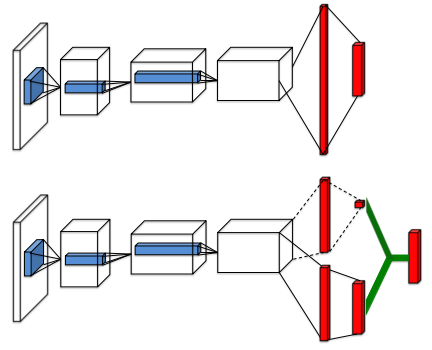
\includegraphics[width=5cm]{pic/dueling-architecture.PNG}
\caption{A popular single stream $Q$-network (\textbf{top}) and the dueling $Q$-network (\textbf{bottom}). The dueling network has two streams to separately estimate (scalar) state-value and the advantages for each action; the green output module implements equation (\ref{dueling_result}) to combine them. Both networks output $Q$-values for each action.} 

\end{figure}
\begin{equation} \label{dueling_result}
Q(s, a; \theta, \alpha, \beta) = V(s; \theta, \beta) + \left(A(s,a;\theta,\alpha) - \frac{1}{|\mathcal{A}|\sum_{a'}{}A(s,a^{'};\theta, \alpha)}\right)
\end{equation}

\paragraph{Experience Replay and Prioritized Experience Replay} Experience Replay  \cite{wang2016sample} has gained popularity in DQN, where it it often motivated as a technique for reducing sample correlation. Experience Replay addresses both of these issue: with experience stored in a replay memory, it becomes possible to break the temporal correlations by mixing more and less recent experience for the updates, and rare experience will be used for more than just a single update. In general, experience replay can reduce the amount of experience required to learn, and replace it with more computation and more memory - which are often cheaper resources that the RL's agent's interactions with its environment. In Experience Replay, the experience transitions were uniformly sampled from a replay memory. the transition are replayed at the same frequency that they were original experienced, regardless of their significance.
and in Prioritized Experience Replay \cite{schaul2015prioritized}, so as to replay important transitions more frequently, and therefore learn more efficiently. and the distributed prioritized experience relpay \cite{horgan2018distributed} the algorithm decouples acting from learning: the actors interact with their own instance of the environment by selecting actions according to a shared neural network, and accumulate the resulting experience in a shared experience replay memory; the learner replays samples of experience and updates the neural network. 

\begin{algorithm}
\caption{Double DQN with proportional prioritization}
\begin{algorithmic}
	\State \textbf{Input}: minibatch $k$, step-size $\eta$, replay period $K$ and size $N$, exponents $\alpha$ and $\beta$, budget $T$.
	\State Initialize replay memory $\mathcal{H}=\Phi, \Delta=0, p_{1}=1$
	\State Observe $S_{0}$ and choose $A_{0} \sim \pi_{\theta}(S_{0})$
	\For {$t = 1$ to $T$}
		\State Observe $S_t, R_t, \gamma_{t}$
		\State Store transition $(S_{t-1}, A_{t-1}, R_{t}, \gamma_t, S_{t})$ with $\mathcal{H}$ with maximal priority $p_{t}=\text{max}_{i<t}p_{i}$
		\If {$t \equiv 0$ mod $K$}
			\For {$j = 1$ to $k$}
				\State Sample transition $j \sim P(j)=p_{j}^{\alpha}/\sum_{i}p_{i}^{\alpha}$
				\State Compute importance-sampling weight $w_{j}=(N \cdot P(j))^{-\beta}/\text{max}_{i}w_{i}$
				\State Compute TD-error $\delta_{j} = R_{j} + \gamma_{j}Q_{\text{target}}(S_{j}, \text{arg max}_{a}Q(S_j, a)) - Q(S_{j-1}, A_{j-1})$
				\State Update transition priority $p_{j} \leftarrow |\delta_{j}|$
				\State Accumulate weight-change $\Delta \leftarrow \Delta + w_{j} \cdot \delta \cdot \nabla_{\theta}Q(S_{j-1}, A_{j-1})$
			\EndFor
			\State Update weights $\theta \leftarrow \theta + \eta \cdot \Delta$, reset $\Delta = 0$
			\State From time to time copy weights into target network $\theta_{\text{target}} \leftarrow \theta$
		\EndIf
		\State Choose action $A_{t} \sim \pi_{\theta}(S_{t})$
	\EndFor
\end{algorithmic}
\end{algorithm}
\paragraph{Distributed Important Sampling} A complementary family of techniques for speeding up training is based on variance reduction by means of \textit{\uline{importance sampling}}. This has been shown be useful in the context of neural networks. Sampling non-uniformly from a dataset and weighting updates according to the sampling probability in order to counteract the bias thereby introduced can increase the speed of convergence by reducing the variance of the gradients. One way of doing this is to select samples with probability proportional to the $L_{2}$ norm of the corresponding gradients. In supervised learning, this approach has been successfully extended to the distributed setting. An alternative is to rank samples according to their latest known loss value and make the sampling probability a function of the rank rather than of the loss itself.
\paragraph{Trust Region Policy Optimization} Trust Region Policy Optimization \cite{Schulman2015Trust, Wu2017Scalable}

\paragraph{Proximal Policy Optimization} Proximal Policy Optimization \cite{Schulman2017Proximal}
\paragraph{Neural Episodic Control} Neural Episodic Control \cite{pritzel2017neural}
Deep reinforcement learning methods attain super-human performance in a wide range of environments. \uline{Such methods are grossly inefficient,  often taking orders of magnitudes more data than human to achieve reasonable performance.} \textcolor{red}{\uline{Neural Episodic Control : a deep reinforcement learning agent that is able to rapidly assimilate new experiences and act upon them. Our agent uses a semi-tabular representation of the value function: a buffer of past experience containing slowly changing state representations and rapidly updated estimates of the value function. }}
\paragraph{} The agent of NEC consists of three components: a convolutional neural network that processes pixel images $s$, a set of memory modules (one per action), and a final network that converts read-outs from the actions memories into $Q(s, a)$ values.
\paragraph{Differentiable Neural Dictionary (DND)} For each action $a \in \mathcal{A}$, NEC has a simple memory module $M_{a} = (K_{a}, V_{a})$, where $K_{a}$ and $V_{a}$ are dynamically sized arrays of vectors, each containing the same number of vectors. The memory module acts as an arbitrary association from keys to corresponding values, much like the dictionary data type found in programs. Thus we refer to this kind of memory module as a \textit{differentiable neural dictionary} (DND). There are two operations possible on a DND: \textit{lookup} and \textit{write}, Performing a lookup on a DND maps a key $h$ to an output value $o$:
\begin{equation} \label{output_o}
o = \sum_{i}w_{i}v_{i}
\end{equation}
where $v_{i}$ is the $i$th element of the array $V_{a}$ and 
\begin{equation} \label{weight_w}
w_{i} = k(h, h_{i})/\sum_{j}k(h, h_{j})
\end{equation}
where $h_{i}$ is the $i$th element of the array $K_{a}$ and $k(x, y)$ is a kernel between vectors $x$ and $y$, e.g., Gaussian or inverse kernels, such as:
\begin{equation}
k(h, h_{i}) = \frac{1}{||h - h_{i}||_{2}^{2} + \delta}
\end{equation}
Thus the output of a lookup in a DND is a weighted sum of the values in the memory, whose weights are given by normalised kernels between the lookup key and the corresponding key in memory. To make queries into very large memories scalable we shall make two approximations in practice: firstly, we shall limit (\ref{output_o}) to the top $p$-nearest neighbours. Secondly, we use an approximate nearest neighbours algorithm to perform the lookups, based up kd-trees.
\paragraph{} keys and values are written to the memory by appending them onto the end of the arrays $K_{a}$ and $V_{a}$ respectively. if a key already exists in the memory, then its corresponding value is updated, rather than being duplicated.
\paragraph{Agent Architecture}
Figure (\ref{nec_agent_architecture_figure}) shows a DND as part of the NEC agent for asingle action, whilst Algorithm (\ref{nec_algorithm}) describes the general outline of the NEC algorithm. 
\paragraph{} The pixel state $s$ is processed by a convolutional neural network to produce a key $h$. The key $h$ is then used to lookup a value from the DND, yielding weights $w_i$ in the process for each element of the memory arrays. Finally, the output is a weighted sum of the values in the DND. The values in the DND, in the case of an NEC agent, are the $Q$ values corresponding to the state that originally resulted in the corresponding key-value pair to be written to hte memory. Thus this architecture produces an estimate of $Q(s, a)$ for a single given action $a$/ The architecture is replicated once for each action $a$ the agent can take, with the convolutional part of the network shared among each separate DND $M_a$. The NEX agent acts by taking the action with the highest $Q$-value estimate at each time step. In practice, we use $\epsilon$-greedy policy during training with a low $\epsilon$.
\begin{figure}
\centering
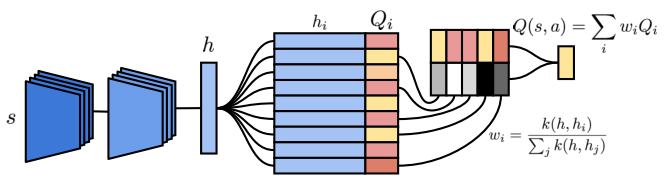
\includegraphics[width=10cm]{pic/nec_agent_architecture.PNG}
\caption{Architecture of episodic memory module for a single action $a$. Pixels representing the current state enter through a convolutional neural network on the bottom left and an estimate of $Q(s, a)$ exists top right. Gradients flow through the entire architecture.} 
\label{nec_agent_architecture_figure}
\end{figure}
\begin{algorithm}
\caption{Neural Episodic Control} \label{nec_algorithm}
\begin{algorithmic}[h]
	\State $\mathcal{D}$: replay memory
	\State $M_{a}$: a DND for each action $a$.
	\State $N$: horizon for $N$-step $Q$ estimate.
	\For {each episode}
		\For {$t = 1, 2, ..., T$}
			\State Receive observation $s_t$ from environment with embedding $h$.
			\State Estimate $Q(s_t, a)$ for each action $a$ via (\ref{output_o}) from $M_{a}$
			\State $a_{t} \leftarrow \epsilon-$greedy policy based on $Q(s_t, a)$
			\State Take action $a_{t}$, receive reward $r_{t+1}$.
			\State Append $(h, Q^{(N)}(s_t, a_t))$ to $M_{a_t}$.
			\State Append $(s_t, a_t, Q^{(N)}(s_t, a_t))$ to $\mathcal{D}$.
		\EndFor
	\EndFor
\end{algorithmic}
\end{algorithm}

\paragraph{}The N-step Q-value estimate is 
\begin{equation} \label{q_n_s_t_a_eq}
Q^{(N)}(s_t, a) = \sum_{j=0}^{N-1}\gamma^{j}r_{t+j} + \gamma^{N}\max_{a^{'}}Q(s_{t+N}, a^{'}).
\end{equation}
The bootstrap term of (\ref{q_n_s_t_a_eq}), $\max_{a^{'}}Q(s_{t+N}, a^{'})$ is found by querying all memories $M_{a}$ for each action $a$ and taking the highest estimated $Q$-value returned. Note that the earliest such values can be added to memory is $N$ steps after a particular $(s, a)$ pair occurs.
\paragraph{}When a state-action value is already present in a DND (i.e the exact same key $h$ is already in $K_a$), the corresponding value present in $V_a, Q_i$, is updated in the same way as the classic tabular Q-learning algorithm:
\begin{equation}\label{update_q_i_eq}
Q_{i}\leftarrow Q_{i} + \alpha(Q^{(N)}(s, a)- Q_{i})
\end{equation}
where $\alpha$ is the learning rate of the $Q$ update.

\ifx\allfiles\undefined
%\bibliographystyle{plain}
\bibliographystyle{unsrt}
\bibliography{reference}
\end{document}
\fi